\chapter{Conclusiones}\label{cap5}

A lo largo de este trabajo se ha descrito el proceso de desarrollo del Sistema AutoSA, en este capítulo se dará cierre al proyecto, comprobando que la implementación del el sistema AutoSA dada en el Capítulo \ref{cap4} satisface los requerimientos funcionales y no funcionales del Capítulo \ref{cap2} sentando así las bases para mostrar el cumplimiento de los objetivos del proyecto AutoSA expresados en el Capítulo \ref{cap1} y enunciar los resultados obtenidos, posteriormente se plantearán posibles mejoras y extensiones al sistema pensando en futuros desarrollos.

\section{Cumplimiento de requerimientos}
El en la sección \ref{sec:req-ana} se expusieron los requerimientos funcionales y no funcionales (secciones \ref{sec:req-fun} y \ref{sec:nonfunctional-req} respectivamente) para el sistema AutoSA. A continuación se verificará el cumplimientos de dichos requerimientos.

\subsection{Cumplimiento de requerimientos funcionales}
La sección \ref{sec:req-fun} lista los requerimientos funcionales del sistema AutoSA, de tales requerimientos se elaboraron los casos de uso, sección \ref{sec:casos-uso}, donde se describen los flujos que debe seguir el sistema AutoSA para cumplir con los requerimientos, es así que a continuación se verifica que la implementación del sistema satisfaga los requerimientos funcionales junto con los casos de uso, además de mostrar la operación del usuario.

\subsubsection{Automatización de los procesos en el Sistema de Abastecimiento}
Los requerimientos funcionales de las secciones \ref{sec:req-contestar} y \ref{sec:req-verificar} automatizan los procesos descritos en la sección \ref{sec:desc-general} y son reflejados en los casos de uso CU-CONTESTAAR y CU-VERIFICAR (ver secciones \ref{cu-contestar} y \ref{cu-verificar} respectivamente), la implementación es mostrada en la sección \ref{sec:agente}. El usuario puede ejecutar las automatizaciones desde la herramienta Sahi de la siguiente forma:
\begin{itemize}
	\item Iniciar Sahi sobre el explorar de Internet (ver punto 1 de la Figura \ref{fig:ss-sahi})
	\begin{figure}[h]
		\centering
		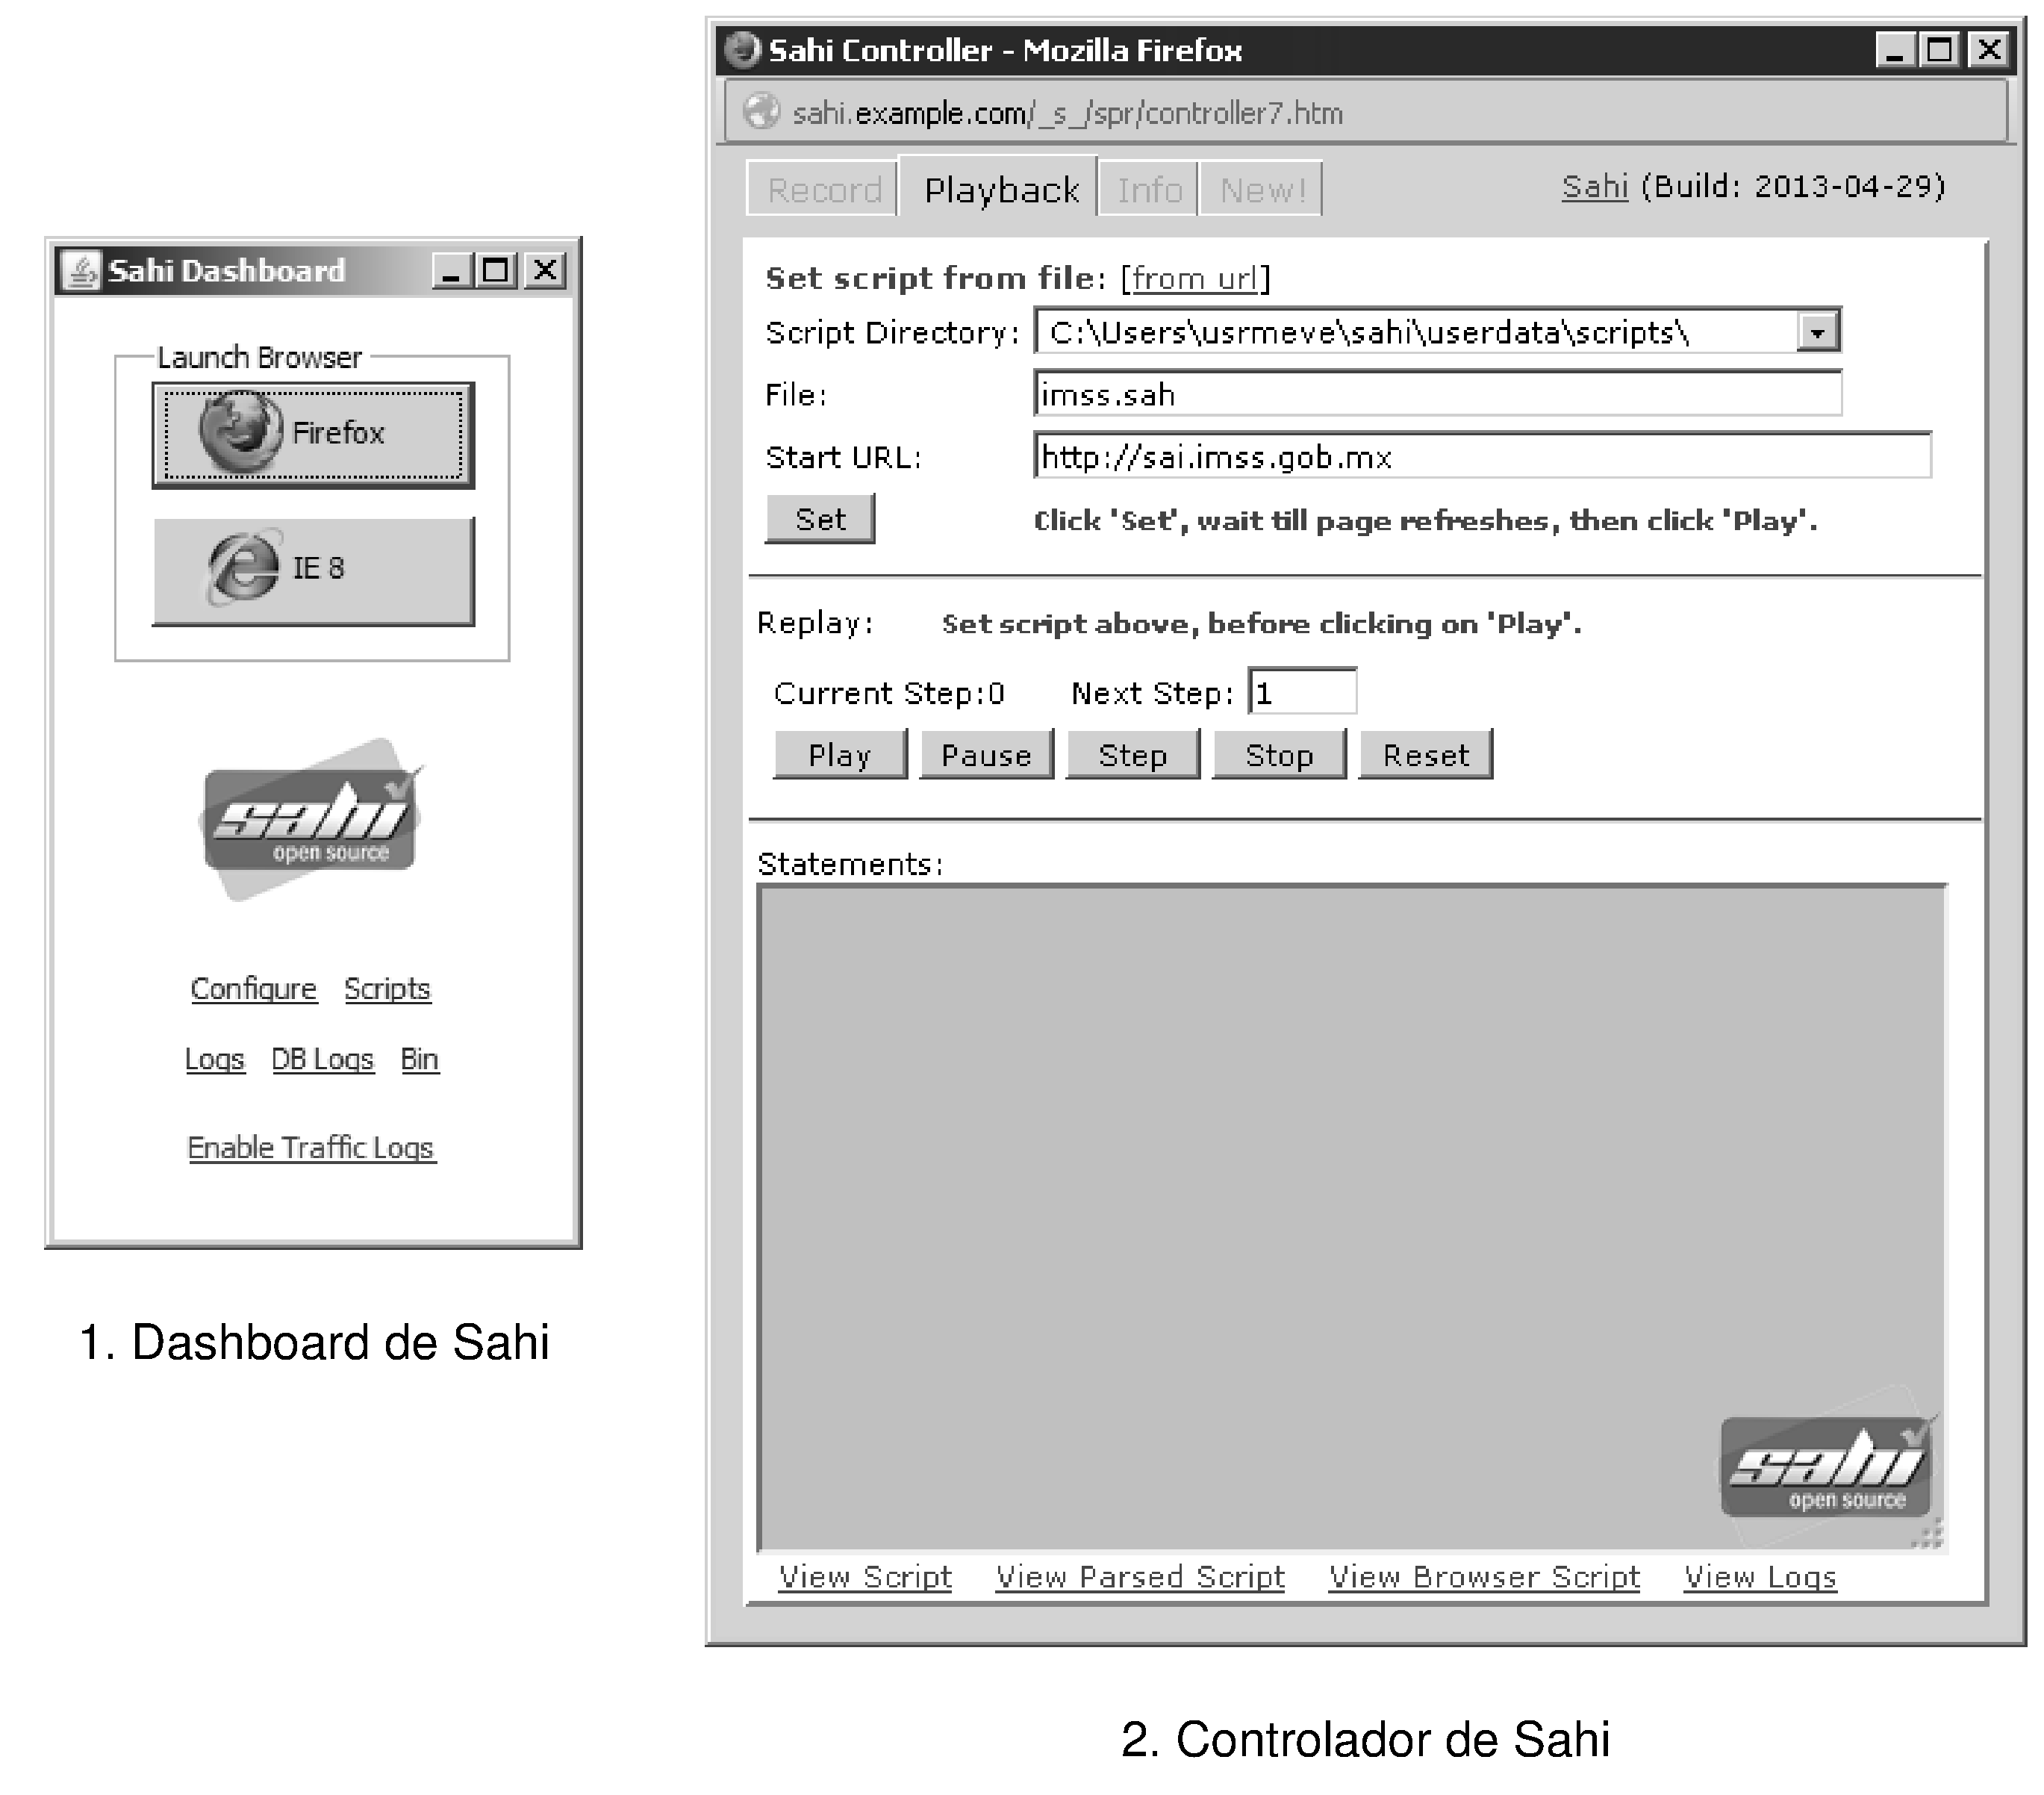
\includegraphics[scale=0.2]{ss-sahi}
		\caption{Interfaz de usuario de Sahi.}
		\label{fig:ss-sahi}
	\end{figure}

	\item Iniciar el controlador de Sahi y hacer los siguientes pasos (ver punto 2 de la Figura \ref{fig:ss-sahi}):
	\begin{enumerate}
		\item Seleccionar la rutina automatizada (contestar órdenes de reposición o verificación de órdenes de reposición)
		\item Ingresar la URL del Sistema de Abastecimiento
		\item Iniciar la ejecución.
	\end{enumerate}
\end{itemize}

\subsubsection{Interfaz WEB para la administración de órdenes de reposición contestadas}
La interfaz Web descrita en este requerimiento (ver sección \ref{sec:req-web-ui}) fue elaborada a lo largo de la sección \ref{sec:web-portal}, en particular los servicios de acceso y autorización fueron mostrados en el apartado 1 de la sección \ref{sec:backend}, así mismo, la pantalla de acceso fue descrita en el apartado 1 de la sección \ref{sec:frontend}.\\
Cabe mencionar que la pantalla de acceso es la primera pantalla que muestra la interfaz Web (ver Figura \ref{fig:ss-login}).
\begin{figure}[h]
	\centering
	\includegraphics[scale=1.8]{ss-login}
	\caption{Captura de pantalla de acceso a la interfaz Web.}
	\label{fig:ss-login}
\end{figure}

\subsubsection{Búsqueda de órdenes de reposición}
La pantalla para la búsqueda de órdenes de reposición es como se muestra al usuario la implementación del requerimiento de la sección \ref{sec:req-search}, la implementación de la pantalla y el comportamiento de están descritos en el apartado 4 de la sección \ref{sec:frontend}. Por otra parte, la implementación de los servicios Web que consume la pantalla de búsqueda de órdenes de reposición es mostrada en el apartado 2 de la sección \ref{sec:backend}.\\
El la Figura \ref{fig:ss-search} se observa la captura de pantalla de búsqueda de órdenes de reposición.
\begin{figure}[h]
	\centering
	\includegraphics[scale=0.4]{ss-search}
	\caption{Captura de pantalla de búsqueda de órdenes de reposición.}
	\label{fig:ss-search}
\end{figure}

\subsubsection{Visualización y edición de una orden de reposición}
Los requerimientos para visualización y edición de una orden de reposición, requerimientos \ref{sec:req-show} y \ref{sec:req-update} respectivamente, son plasmados en los casos de uso CU-VISUALIZAR y CU-EDITAR (secciones \ref{cu-visualizar} y \ref{cu-editar} respectivamente). En la implementación y en la interfaz de usuario se utiliza la misma pantalla, como se muestra en la Figura \ref{fig:ss-edit}, esta vista es descrita en el apartado 5 de la sección \ref{sec:frontend}. La implementación de los servicios Web que consume la pantalla son mostrados en el apartado 2 de la sección \ref{sec:backend}.
\begin{figure}[h]
	\centering
	\includegraphics[scale=0.4]{ss-edit}
	\caption{Captura de pantalla de búsqueda de órdenes de reposición.}
	\label{fig:ss-edit}
\end{figure}

\subsubsection{Generación de reportes}
La generación de reportes cumple con los requerimientos de las secciones \ref{sec:req-rep-contestadas}, \ref{sec:req-rep-layout} y \ref{sec:req-rep-canceladas}; mismos que son englobados en el caso de uso CU-GENERAR-REPORTE (ver sección \ref{cu-generar-reporte}). La implementación de la generación de reportes está descrita en la sección \ref{sec:gen-repport} y, a su vez, los servicios Web que exponen esta funcionalidad están en el apartado 2 de la sección \ref{sec:backend}. La vista que se muestra al usuario se encuentra en el apartado 2 de la sección \ref{sec:frontend}, en la Figura \ref{fig:ss-report} se observa la captura de pantalla como se muestra al usuario\footnote{Por acuerdo de confidencialidad no se puede mostrar el contenido de los reportes generados.}. 
	\begin{figure}[h]
		\centering
		\includegraphics[scale=0.5]{ss-report}
		\caption{Captura de pantalla de generación de reportes.}
		\label{fig:ss-report}
	\end{figure}

\subsubsection{Actualización de catálogos y estatus de órdenes de reposición canceladas}
Los requerimientos \ref{sec:req-catalogos} y \ref{sec:req-canceladas} son modelados en el caso de eso CU-ACTUALIZAR-CATALOGO (ver sección \ref{cu-actualizar-catalogo}), la implementación de la actualización a los datos es dada en la sección \ref{sec:persistence-web}, y la implementación del servicio Web se encuentra en el apartado 2 de la sección \ref{sec:backend}. La implementación de la vista está dada en el apartado 3 de la sección \ref{sec:frontend}, en la Figura \ref{fig:ss-catalog} se observa la captura de pantalla de la administración de catálogos\footnote{Por acuerdo de confidencialidad no se puede mostrar el contenido de los catálogos.}.
\begin{figure}[h]
	\centering
	\includegraphics[scale=0.4]{ss-catalog}
	\caption{Captura de pantalla de administración de catálogos.}
	\label{fig:ss-catalog}
\end{figure}

\subsubsection{Navegación dentro de la interfaz web}
La implementación del requerimiento \ref{sec:req-nav-bar} es mostrada en la sección \ref{sec:frontend}, en la Figura \ref{fig:ss-nav-bar} se observa la captura de pantalla de la barra de navegación.
\begin{figure}[h]
	\centering
	\includegraphics[scale=0.4]{ss-nav-bar}
	\caption{Captura de pantalla de la barra de navegación.}
	\label{fig:ss-nav-bar}
\end{figure}


\subsection{Cumplimiento de requerimientos no funcionales}
En la sección \ref{sec:nonfunctional-req} se enlistan los requerimientos no funcionales para el sistema AutoSA.

\subsubsection{Ejecución del Sistema AutoSA en los sistemas operativos más comunes.}
En la sección \ref{sec:java} se menciona que el lenguaje de programación Java es multiplataforma gracias a que el código escrito por los desarrolladores es traducido a \consolatext{bytecode} y es este último el que ejecuta la máquina virtual de Java. Existen implementaciones de robustas y ampliamente probadas de la máquina virtual de Java para una gran variedad de sistemas operativos, es por esta razón que se decidió utilizar a Java como el lenguaje de programación principal.

\subsubsection{Base de datos relacional SQL}
Al principio del proyecto, la farmacéutica sentó que de ser necesaria una base de datos, el área encargada de las bases de datos de la farmacéutica sería quien daría la infraestructura y la base de datos provista sería relacional por lo que las rutinas DDL y DML de la sección \ref{sec:impl-db} y las consultas del módulo de persistencia (ver sección \ref{sec:persistence}) siguen los estándares SQL mostrados en la sección \ref{sec:bd-r}.

\subsubsection{Uso de la herramienta Sahi para automatizar interacción con Sistema de Abastecimiento}
En el cumplimiento de los requerimientos funcionales 1 y 2 de la sección anterior y en la sección \ref{sec:agente} se muestra la implementación del módulo \textbf{Agente} utilizando Sahi.

\subsubsection{Las contraseñas de los usuarios para el acceso a la interfaz web deben ser almacenadas utilizando un algoritmo de cifrado}
En la sección \ref{sec:backend} se muestra la verificación y cifrado de la contraseña de un usuario.


\section{Resultados}
El objetivo principal del proyecto AutoSA, definido en la sección \ref{sec:objetivo-principal}, es automatizar la interacción de los operadores de la farmacéutica con el Sistema de Abastecimiento para contestar y verificar órdenes de reposición del Instituto de Salud. En las primeras semanas desde la liberación del sistema AutoSA se contestaron exitosamente la totalidad de las órdenes de reposición, que en promedio son 400 órdenes por día, el tiempo de atención promedio fue de hora y media. Cabe resaltar que hasta la fecha no se han reportado defectos graves o críticos, así como errores en los datos de la respuesta a las órdenes de reposición. Por lo anterior se puede concluir que el proyecto AutoSA ha cumplido con el objetivo para el cuál fue propuesto. Posterior a la liberación del sistema AutoSA la consultara dueña del desarrollo del sistema AutoSA ha implantado el sistema AutoSA en otras compañías farmacéuticas teniendo resultados a los obtenidos en la primera compañía farmacéutica.\\

El uso del sistema AutoSA trajo con sigo los beneficios esperados (ver sección \ref{sec:objetivos-secundarios}):
\begin{enumerate}
	\item Reducción de tiempo en cuanto a la respuesta de órdenes de reposición, previo al uso del sistema AutoSA, a los operadores de la farmacéutica les tomaba 24 horas hombre al día contestar 400 órdenes de reposición en un día, con el sistema AutoSA el tiempo de respuesta bajó a 1.5 horas, este hecho ocasionó que todo el proceso de la compañía farmacéutica para entregar el medicamento desde que se publicaron las órdenes de reposición en el Sistema de Abastecimiento bajara de uno a dos días.
	\item Reducción de horas extras en las jornadas laborales de los operadores de la compañía farmacéutica, debido al ahorro de tiempo en la respuesta a las órdenes de reposición, los operadores pueden realizar sus tareas diarias dentro de la jornada laboral de 8 horas.
	\item Reducción del error humano en relación a la manipulación de la información, hasta la fecho no se han reportado errores o inconsistencias en los datos de las respuestas a las órdenes de reposición.
	\item Consistencia en los datos respecto a la generación de reportes estadísticos sobre las órdenes de reposición procesadas, del punto anterior es sabido que no existen inconsistencias en los datos de las órdenes de reposición almacenados en la base de datos por lo que los reportes estadísticos muestran datos consistentes y verdaderos.
	\item Ahorro de recursos en la entrega de medicamentos no solicitados, se redujo la entrega de medicamento no solicitado, la información exacta de esta reducción no ha sido compartido por la compañía farmacéutica.
\end{enumerate}


\section{Trabajo futuro}
\begin{itemize}
	\item Actualizar bibliotecas, marcos de trabajo y ambientes versiones actuales: han pasado más de 3 años desde la liberación.
	\item Ejecución en paralelo, acondicionar el sistema AutoSA para ejecutar la rutina automatizada para contestar órdenes de reposición en varias instancias de la herramienta Sahi con el fin de reducir aún más el tiempo de respuesta a las órdenes de reposición.
	\item Extender el alcance del sistema para interactuar con el sistema de la farmacéutica que maneja el inventario de la bodega de medicamentos, esto quiere decir que al terminar la atención de las órdenes de reposición el sistema AutoSA enviaría el reporte de los medicamentos solicitados directamente a la bodega agilizando así el proceso de entrega de medicamentos a los centros de salud. 
	\item Ejecución automática de las rutinas de automatizadas, dar la posibilidad a los usuarios de programar el momento del día en que se ejecuten las rutinas automatizadas, de esta forma no se necesitaría un operador que iniciara manualmente las rutinas automatizadas.
\end{itemize}

\section{Conclusiones finales}
En el desarrollo de este proyecto y en toda mi carrera profesional he aplicado conocimientos que adquirí en la Facultad de Ciencias sobre programación y paradigmas de programación, lógica, bases de datos, redes de computadoras, ingeniería de software, análisis y diseño de algoritmos, teoría de códigos, álgebra lineal. De igual manera también he utilizado las habilidades y costumbres que adquirí como alumno de la licenciatura en Ciencias de la Computación: buscar y aprender por mi mismo nuevas tecnologías, pensar soluciones alternativas. Todo esto (conocimientos, habilidades y costumbres) me ha apoyado para mantenerme en constante actualización y ser un profesional competente en los equipos de trabajo de los cuales he formado parte.\\
Este reporte a mostrado el desarrollo del proyecto AutoSA por las etapas, cuya responsabilidad recayó en mi persona, bajo la supervisión de un arquitecto de software de la compañía en la cual se desarrolló este proyecto:
\begin{itemize}
 	\item Presentación del problema y propuesta de solución, capítulo \ref{cap1}. 
 	\item Análisis de requerimientos y creación de casos de uso, capítulo \ref{cap2}.
 	\item Diseño de arquitectura y componentes, capítulo \ref{cap3}.
 	\item Implementación de los componentes, capítulo \ref{cap4}.
\end{itemize} 
Durante todas estas etapas se trabajó en constante comunicación con los operadores de la farmacéutica, en primer lugar para copiar exactamente la interacción con el Sistema de Abastecimiento del Instituto de Salud. Posteriormente para la ejecución de pruebas de las rutinas automatizadas, pues al no tener un ambiente en el Sistema de Abastecimiento en el cual realizar pruebas, estás fueron realizadas directamente en producción, entonces la supervisión de los operadores fue necesaria para asegurar que ninguna orden de reposición no fuera atendida por parte de la farmacéutica y además garantizar que los datos de las órdenes fueran almacenados correctamente, que la generación de los acuses de envió fuera correcta así como el contenido del reporte de órdenes atendidas necesario para seguir la atención de las órdenes por parte de otras áreas de la compañía farmacéutica.\\
El resultado del proyecto AutoSA es un sistema robusto, que si bien tiene puntos mejora, al día de hoy no ha presentado fallos graves o críticos, ha cubierto las necesidades de la compañía farmacéutica superando el ahorro de tiempo previsto, ha reducido costos por errores humanos y costos por errores en logística, además evitar a los operadores de la farmacéutica jornadas laborales de 10 horas.\\
El proyecto AutoSA ha mostrado ser de utilidad en la industria farmacéutica, tan es así que tras el uso exitoso en la compañía farmacéutica para la cual se desarrolló este proyecto, el sistema AutoSA ha sido requerido por otras compañías farmacéuticas y hasta hoy sigue siendo  utilizando diariamente.
